This section explains the concept of parameter graphs that are used to encode
the parameter space of solvers in EDACC. If you are only interested in specifying the parameter space
of a solver we suggest to skim over the details and first take a look at the example \ref{paramspecexample}.
In the context of parameter spaces a parameter is an input variable of a program and is defined by a name and a domain.
Properties of parameters such as the command line prefix and the order in which the should appear when calling the solver executable
aren't of interest in this context.

\begin{definition}
A domain defines the set of possible values that can be assigned to a parameter (in a solver configuration). It can be one of the following or the union (which we call mixed domain) of any number of them (except for the flag domain, which can only occur on its own).
\begin{enumerate}
\item real: values between a lower and an upper bound
\item integer: values between a lower and an upper bound
\item ordinal: list of values in a min to max order
\item categorial: set of possible values
\item optional: consists only of a special value "not specified"
\item flag: consists of two special values "on" and "off" (for parameters that are flags, i.e. present or not)
\end{enumerate}
\end{definition}

\begin{definition}
The parameter space of a solver is defined by its parameters and their possible values. The parameter space can be further constrained by
dependencies between parameters such as
\begin{enumerate}
\item Parameter X can be specified if parameter Y takes on certain values
\item Parameter X has to be specified if parameter Y takes on certain values
\item Parameter X has to take on certain values depending on the values of parameters Y, Z, ...
\end{enumerate}
\end{definition}

There are several problems that come up in the context of EDACC: Determine if a given solver configuration is valid, i.e. in the solver's parameter space.
Given the parameter space, construct a valid solver configuration. Given a valid solver configuration, find a ''neighbouring'' solver configuration that is also valid.

\begin{definition}
A parameter graph is a directed, acyclic graph that represents the parameter space. It consists of AND-Nodes and OR-Nodes and edges between them. Edges are directed and allowed only
between different types of nodes. OR-Nodes can have multiple incoming edges, while AND-Nodes can only have exactly one incoming edge. Additionally edges have a group number which is 0 if the edge doesn't belong to any group.
Parameter graphs have a single unique AND-Node without any incoming edges. This node will be referred to as start node.
\end{definition}

\begin{definition}
OR-Nodes have a reference to a parameter.
\end{definition}

\begin{definition}
AND-Nodes have a domain and a parameter reference to the same parameter as the preceding OR-node.
AND-Nodes partition the possible values of the parameter that they (and the preceding OR-node) reference.
The domain of an AND-Node has to be a subset of the domain of the preceding OR-Node.
\end{definition}

The general idea is that the parameter space is specified by following the structure of the graph from the start node and constraining the parameters using the domains encountered
on the nodes.
AND-Nodes imply that all outgoing edges have to be followed while OR-Nodes mean that exactly one edge has to be followed.

More formally:
\begin{definition}
A solver configuration is valid if the start node (an AND-Node) of the parameter graph is satisfied. Satisfied means:
\begin{enumerate}
\item an AND-Node is satisfied if the corresponding parameter value lies in its domain and all OR-nodes adjacent via ungrouped edges are satisfied.
\item an OR-Node is satisfied if exactly one adjacent AND-Node is satisfied and for at least one set of incoming edges with common group number the preceding AND-Nodes are all satisfied.
\end{enumerate}
\end{definition}

\clearpage

\subsection{Example}
\label{paramspecexample}
\marginlabel{\Eexample}
Consider a solver that has the following parameters:
\begin{itemize}
\item \textit{c1} which takes on integer values in $[1,10]$.
\item \textit{ps} which takes on real values in $[0,1]$.
\item A flag called \textit{lookahead} which can be present or not.
\item A categorical parameter \textit{steps} which takes on values in $\{0,1,2,3,4\}$.
\item Another categorical parameter \textit{method} whose value is either ''hybrid'' or ''atom''.
\item A parameter \textit{prob} which can be left out or take on real values in $[0,1]$.
\end{itemize}
Furthermore there are some restrictions and requirements:
\begin{itemize}
\item Both \textit{c1} and \textit{ps} have to be always specified.
\item If the \textit{lookahead} flag is present, both \textit{steps} and \textit{method} have to be present.
\item If \textit{steps} takes on the value $0$ and \textit{method} takes on the value ''hybrid'', then the parameter \textit{prob} can take on values in its real domain $[0,1]$ or be left out.
\end{itemize}
This parameter space can be encoded in a parameter graph as defined earlier in the following way:
\begin{figure}[htb]
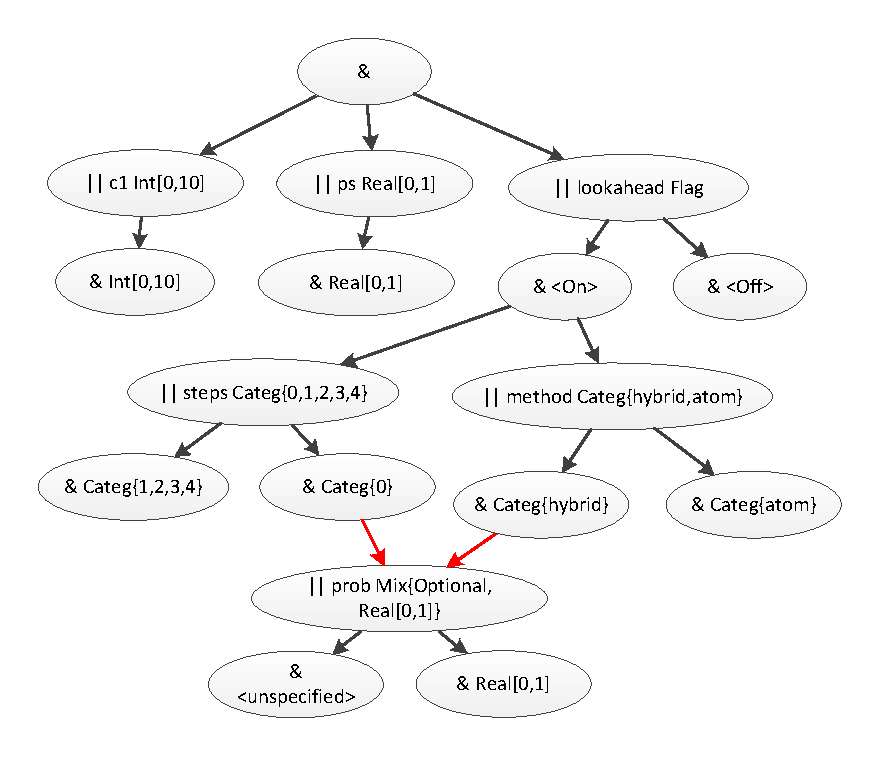
\includegraphics[width=10cm]{paramgraph.pdf}
\end{figure}

The two red edges imply the membership of the edges to the same edge group $\neq 0$. Black edges mean that the edge doesn't belong to any group.
For simplicity, the parameter references of AND-Nodes (to the same parameter as the preceeding OR-Node) are not shown in the graph.

